\documentclass[tikz,border=8pt]{standalone}
\usepackage{amsmath}
\usepackage{pgfplots}
\pgfplotsset{compat=1.18}
\usetikzlibrary{arrows.meta}
\definecolor{ink}{HTML}{21352F}
\definecolor{teal}{HTML}{087F7B}
\definecolor{blue}{HTML}{4B77A8}
\definecolor{gold}{HTML}{C58B2A}
\definecolor{rose}{HTML}{B65A62}
\begin{document}
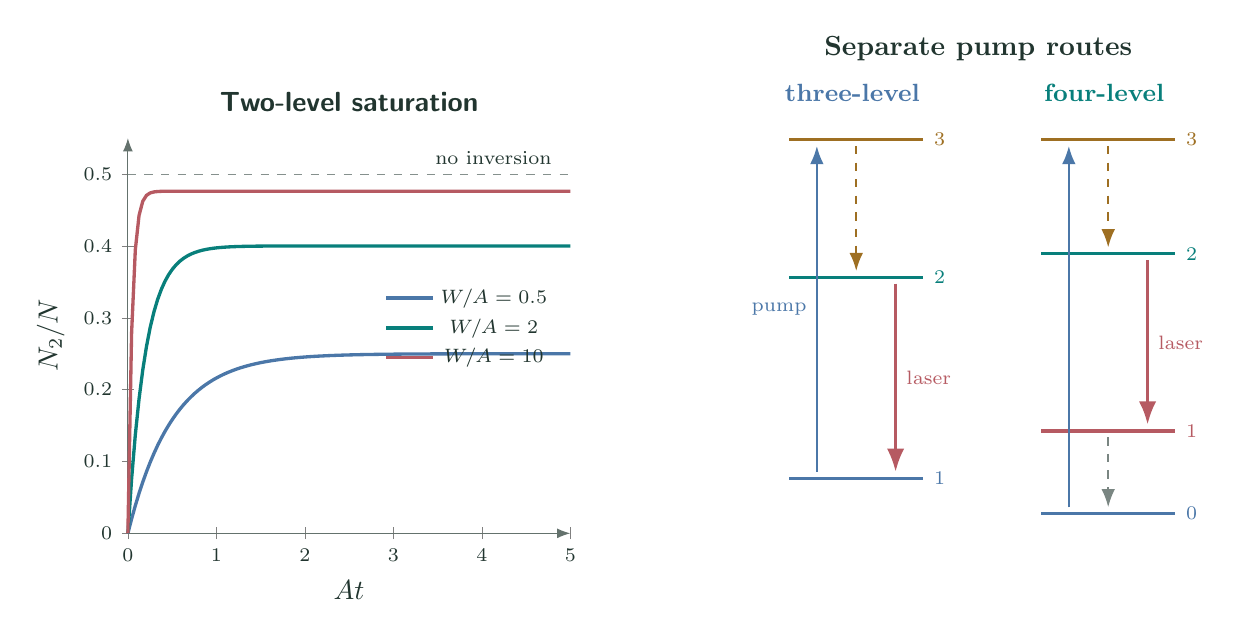
\begin{tikzpicture}[font=\sffamily,text=ink,>=Latex]
  \begin{axis}[
    at={(0cm,0cm)},anchor=south west,
    width=7.2cm,height=6.6cm,
    xmin=0,xmax=5,ymin=0,ymax=.55,
    axis lines=left,
    axis line style={draw=ink!70,->},
    xlabel={$At$},ylabel={$N_2/N$},
    title={\bfseries Two-level saturation},
    legend style={draw=none,fill=none,font=\scriptsize,
      at={(.98,.52)},anchor=east},
    tick label style={font=\scriptsize},
    clip=false
  ]
    \addplot[blue,very thick,domain=0:5,samples=120]
      {(.5/(2*.5+1))*(1-exp(-(2*.5+1)*x))};
    \addlegendentry{$W/A=0.5$}
    \addplot[teal,very thick,domain=0:5,samples=120]
      {(2/(2*2+1))*(1-exp(-(2*2+1)*x))};
    \addlegendentry{$W/A=2$}
    \addplot[rose,very thick,domain=0:5,samples=120]
      {(10/(2*10+1))*(1-exp(-(2*10+1)*x))};
    \addlegendentry{$W/A=10$}
    \addplot[ink!55,dashed,domain=0:5] {.5};
    \node[font=\scriptsize,anchor=south east] at (axis cs:4.9,.5)
      {no inversion};
  \end{axis}

  \begin{scope}[xshift=8.4cm]
    \node[font=\bfseries] at (2.4,6.15)
      {Separate pump routes};

    \node[font=\small\bfseries,text=blue] at (0.8,5.6)
      {three-level};
    \draw[blue,very thick] (0,0.7)--(1.7,0.7)
      node[right,font=\scriptsize] {$1$};
    \draw[teal,very thick] (0,3.25)--(1.7,3.25)
      node[right,font=\scriptsize] {$2$};
    \draw[gold!80!black,very thick] (0,5.0)--(1.7,5.0)
      node[right,font=\scriptsize] {$3$};
    \draw[blue,->,thick] (.35,.78)--(.35,4.92)
      node[midway,left,font=\scriptsize] {pump};
    \draw[gold!80!black,->,thick,dashed] (.85,4.92)--(.85,3.33);
    \draw[rose,->,very thick] (1.35,3.17)--(1.35,.78)
      node[midway,right,font=\scriptsize] {laser};

    \node[font=\small\bfseries,text=teal] at (4.0,5.6)
      {four-level};
    \draw[blue,very thick] (3.2,0.25)--(4.9,0.25)
      node[right,font=\scriptsize] {$0$};
    \draw[rose,very thick] (3.2,1.3)--(4.9,1.3)
      node[right,font=\scriptsize] {$1$};
    \draw[teal,very thick] (3.2,3.55)--(4.9,3.55)
      node[right,font=\scriptsize] {$2$};
    \draw[gold!80!black,very thick] (3.2,5.0)--(4.9,5.0)
      node[right,font=\scriptsize] {$3$};
    \draw[blue,->,thick] (3.55,.33)--(3.55,4.92);
    \draw[gold!80!black,->,thick,dashed] (4.05,4.92)--(4.05,3.63);
    \draw[rose,->,very thick] (4.55,3.47)--(4.55,1.38)
      node[midway,right,font=\scriptsize] {laser};
    \draw[ink!60,->,thick,dashed] (4.05,1.22)--(4.05,.33);
  \end{scope}
\end{tikzpicture}
\end{document}
